Il progetto PRISMA si articola in una complessa struttura che si sviluppa tra diverse componenti software e architetturali. Nelle sottosezioni a seguire verranno illustrati quelle principali con cui si è interagito o che si sono adoperate lungo lo svolgimento del progetto.

\subsection{Framework N3} \label{framework-N3}

\begin{wrapfigure}{r}{0.3\textwidth}
    \vspace{-34pt}
    \begin{center}
    
\includegraphics[width=0.3\textwidth]{images/logo_orma.png}
    \end{center}
    \vspace{-30pt}
\end{wrapfigure}
Nella sezione \ref{software} si è accennato all'uso di PHP e JavaScript con alcuni relativi framework. Tra di essi si annovera il framework sviluppato dall'azienda N3 con cui è avvenuta la collaborazione del progetto: \textbf{Orma - \emph{Management System}}.
Il framework si avvale di PHP (e Symfony), JavaScript e DataTables, è modellato su un \textbf{pattern MVC} ed è orientato all'interazione con gli oggetti, che possono essere visualizzati, aggiunti, modificati o cancellati, mediante una visualizzazione tabellare. 
Originariamente si basava sull'interazione con un database, ma in questo caso è stato adattato per lavorare con i dati presenti sul \textbf{file system} del nodo; inoltre nonostante si sia preservata la struttura base è stato necessario, data la complessità del progetto, svincolare da alcuni paradigmi lungo lo sviluppo del sito. La struttura del framework è molto complessa, si presentano qui dunque i dettagli più importanti per comprenderne il funzionamento generale.

Il framework è stato progettato per gestire un insieme di \textbf{oggetti} con cui l'utente può interagire.
Impone quindi la realizzazione di una web application divisa in diverse \textbf{sezioni}, ciascuna delle quali è inerente ad una classe di oggetti presente sul database (o file system). Su ogni oggetto possono essere effettuate varie \textbf{operazioni}:
\begin{itemize}[noitemsep,nolistsep]
    \item \textbf{Visualizzazione} (\emph{get})
    \item \textbf{Inserimento} (\emph{insert})
    \item \textbf{Modifica} (\emph{edit})
    \item \textbf{Cancellazione} (\emph{delete})
\end{itemize}

\subsubsection{Lato client}

Ad ogni operazione su ciascuna classe di oggetti è associata una pagina HTML diversa, a cui si ha accesso tramite una gestione a \textbf{controller}, secondo il paradigma di Symfony. Accedendo a ciascuna sezione secondo i collegamenti predisposti graficamente, i controller reindirizzano l'utente a URL specifici a seconda dell'operazione che è richiesta eseguire sull'oggetto, occupandosi di gestire anche una prima parte di sicurezza degli accessi. 

Nella seguente spiegazione del flusso dell'applicazione ci si sofferma soprattutto sull'operazione di \textbf{modifica}, siccome è l'unica utilizzata nell'applicazione illustrata.

Per ogni sezione è presente una pagina di script JS (chiamata come la classe dell'oggetto, le classi degli oggetti si chiamano invece con il nome della classe e il suffisso \texttt{Class}), che gestisce gli eventi diretti generati dalle interazioni dell'utente con il sito e le operazioni principali con appositi metodi (ad esempio, \texttt{editObj()} per la modifica). Ciascuna sezione mostra una \textbf{tabella}, realizzata con DataTables, che elenca gli oggetti della classe con i rispettivi attributi presenti del database. Ad esempio, la sezione \emph{Utenti} avrà una tabella con una riga per ogni utente presente nel DB e due colonne che corrisponderanno a username e livello, ovvero gli attributi dell'utente. Inoltre sotto la tabella è presente un \emph{form} con tanti campi quanti sono gli attributi dell'oggetto: cliccando sulla riga corrispondente, il sistema riempie automaticamente i campi con gli attributi esistenti e l'utente ha la possibilità di modificarli e inviare le modifiche. 

Le operazioni sugli oggetti prima di essere inviate come richieste al server passano attraverso una complessa pipeline.
Si deve dunque implementare per ciascuna classe di oggetti una classe che mandi le informazioni da elaborare allo script \texttt{form.js} (che si chiamerà con il nome della classe con il suffisso \texttt{Logic}) e una classe che riceve i dati elaborati da quest'ultimo e interagisca con il server (che avrà il nome della classe con l'aggiunta del suffisso \texttt{Factory}). Le classi \texttt{-Logic} sono particolari perché contengono un unico dizionario le cui chiavi sono le classi e i valori le funzioni chiamate nello script \texttt{form.js}.

Lo script \texttt{form.js} ha il compito di gestire il riempimento dei campi nel form di modifica, la validazione dei campi attraverso un apposito sistema di validazione, la distinzione delle operazioni (ad esempio se l'utente ha richiesto la modifica di un oggetto esistente oppure l'aggiunta di uno nuovo), la visualizzazione di messaggi di successo o di errore, l'aggiornamento delle tabelle e così via.

Le classi \texttt{-Factory} interagiscono infine con un'ultima classe che contiene dei metodi appositi per eseguire le chiamate AJAX al server.

\subsubsection{Lato server}

Per quanto riguarda il server, la logica è divisa anche in questo caso ad oggetti. Ciascun oggetto è gestito da un insieme di classi PHP che ricevono le richieste e operano sul database.

In particolar modo, gli endpoint delle richieste sono gestiti con il micro-framework Silex. Ogni endpoint è relativo ad una singola operazione o alla generazione di una tabella. Similmente al lato client, dal file \emph{index} l'operazione da eseguire attraversa una pipeline composta da diverse classi fino alla creazione di una query da effettuare sul database. Siccome il progetto non si affidava ad un database, si tralascia la spiegazione dettagliata della pipeline, la maggior parte del lavoro si è focalizzato su un'unica classe in cui implementare i metodi necessari.

\subsubsection{Modifiche al framework}

Dal momento che il progetto PRISMA è più complesso e non necessita di una semplice gestione di oggetti su database, sono state apportate delle modifiche e delle integrazioni:
\begin{itemize}
    \item Si è introdotto il caricamento/scaricamento di file e immagini indipendenti dai singoli oggetti;
    \item Si sono implementate delle sezioni non inerenti a classi di oggetti, ad esempio la sezione relativa alla VPN (cfr. sezione \ref{sezione-OVPN});
    \item Si è resa necessaria l'integrazione per interagire con il file system del nodo dal momento che il framework era stato progettato per lavorare su un database; di conseguenza è stata rimossa la pipeline per la formulazione di query e si sono implementati metodi per leggere e scrivere direttamente sul file system.
\end{itemize} 

\subsection{Configurazione della macchina} \label{debian}

Su tutti i nodi è installato come sistema operativo \textbf{Debian Bullseye 11.2}.
Una volta che si è configurato il sistema operativo ci si può collegare alla macchina in SSH per installare tutti i software necessari. Nelle sottosezioni a seguire si approfondiranno le configurazioni principali.

Per quanto riguarda i software di base da installare tra i più importanti si citano Git, OpenVPN, SSH, Docker (secondo il manuale ufficiale \cite{install-Docker-Debian}) e \emph{Prometheus Node Exporter} v1.3.1 (scaricabile dal repository GitHub ufficiale \cite{Prometheus-node-exporter-github} e configurato secondo la guida ufficiale \cite{Prometheus-node-exporter}). Si installano poi i driver della scheda di rete e si effettua la configurazione mDNS per risolvere \texttt{'prismanode.local'} con l'ip del nodo.

Si prosegue quindi importando i file script programmati per bash, finalizzati alla corretta inizializzazione dei container (cfr. sezione \ref{docker}), i sorgenti base dell'applicazione e le chiavi private SSH. A questo punto è possibile accedere tramite browser alla schermata di login dell'applicazione (cfr. sezione \ref{accesso-app}) inserendo l'IP del nodo. Sulla porta 9090 è inoltre possibile accedere all'interfaccia grafica di \emph{Prometheus Node Exporter}. 

Nel corso del tirocinio sono state apportate inoltre delle modifiche alla configurazione iniziale della macchina (cfr. sezione \ref{permessi-macchina}).

\subsection{Rete VPN} \label{rete-VPN}

Il nodo è inserito durante la pre-produzione in una VPN provvisoria, \emph{VPN Guest}, con indirizzo IP provvisorio. Una volta che è stato configurato viene collegato invece alla VPN effettiva, comune a tutti i nodi, con indirizzo IP fisso.
Tutte le configurazioni VPN appena illustrate sono realizzate con \textbf{OpenVPN} \cite{OpenVPN}.

L'utente una volta che si collega in VPN può accedere a tutti i nodi in SSH oppure tramite la web application qui discussa, se ne conosce l'indirizzo IP.

\subsection{FreeTure} \label{freeture}

Per riprendere e individuare gli eventi atmosferici, PRISMA si appoggia a \textbf{FreeTure} \cite{FreeTure}, un software open source di rilevamento di meteore usato per monitorare il cielo con camere all-sky GigE per rilavare e registrare stelle cadenti e fireball.
Il software genera immagini in formato FITS \cite{FITS}, fornisce la possibilità di eseguire acquisizioni a lunga esposizione regolari o programmate ed infine dà la possibilità di accumulare fotogrammi per tenere una sorta di cronologia. 

La telecamera del nodo dipende pertanto dalla configurazione FreeTure (i dati di configurazione sono riportati in un unico file) situata in un apposito container (cfr. sezione \ref{docker}), che definisce, tra i valori più degni di nota, le modalità di acquisizione delle immagini, le interazioni con il file system, la calibrazione della telecamera e l'elaborazione degli scatti per l'individuazione di eventi.

\begin{lstlisting}[style=PHP,caption={Parte della configurazione FreeTure che risiede sul nodo di Codogno.},captionpos=b]
[...]
# Name of the station.
STATION_NAME = CODOGNO	
# Station name.
TELESCOP = ITLO06
# Person in charge.
OBSERVER = Eng. Andrea Novati
# Instrument name.
INSTRUME = FREETURE-CAM
# Camera model name.
CAMERA = BASLER1300gm
# Camera focal.
FOCAL = 1.25
# Camera aperture.
APERTURE = 2.0
# Longitude observatory.
SITELONG = 9.6909138
# Latitude observatory.
SITELAT = 45.1638302
# Elevation observatory.
SITEELEV = 58
[...]
\end{lstlisting}

Inoltre, è possibile definire un file formato BMP che si comporta da “maschera” nell'inquadratura della telecamera: qualsiasi evento che si trovi al di fuori della maschera viene ignorato.

\subsection{Architettura dei container e dei volumi} \label{docker}

Sulla macchina associata alla telecamera è installato \textbf{Docker} \cite{Docker}, che gestisce un insieme di container. Nella figura \ref{fig:containers-arch} sono mostrati i vari container e le interazioni tra di essi. 

L'utente accede al nodo tramite VPN Guest o con VPN di produzione in SSH sulla porta 20, oppure tramite la web application sulla porta 80, realizzata con un web server Apache collocato nel container \emph{prisma-orma}\footnote{L'immagine del container è reperibile su Docker Hub \cite{orma-webmin}}. Da quest'ultimo container, è possibile ugualmente accedere in SSH all'host stesso, da cui si può modificare la configurazione VPN (legata all'host e non ai container). 

A questi container, sono associati dei volumi che mappano delle cartelle sull'host: in \emph{orma-src} sono presenti i sorgenti per la web application, mentre in \emph{orma-keys} è presente la parte relativa agli utenti che possono accedere alla web application.

Inoltre tramite server web si può accedere al volume dove risiede la configurazione FreeTure (\emph{freeture-conf}) e a quello dove sono memorizzati i dati raccolti dalla telecamera (\emph{freeture-data}).
Con questi ultimi due volumi interagisce il container \emph{freeture}, legato alla telecamera.

\begin{figure}
\begin{center}
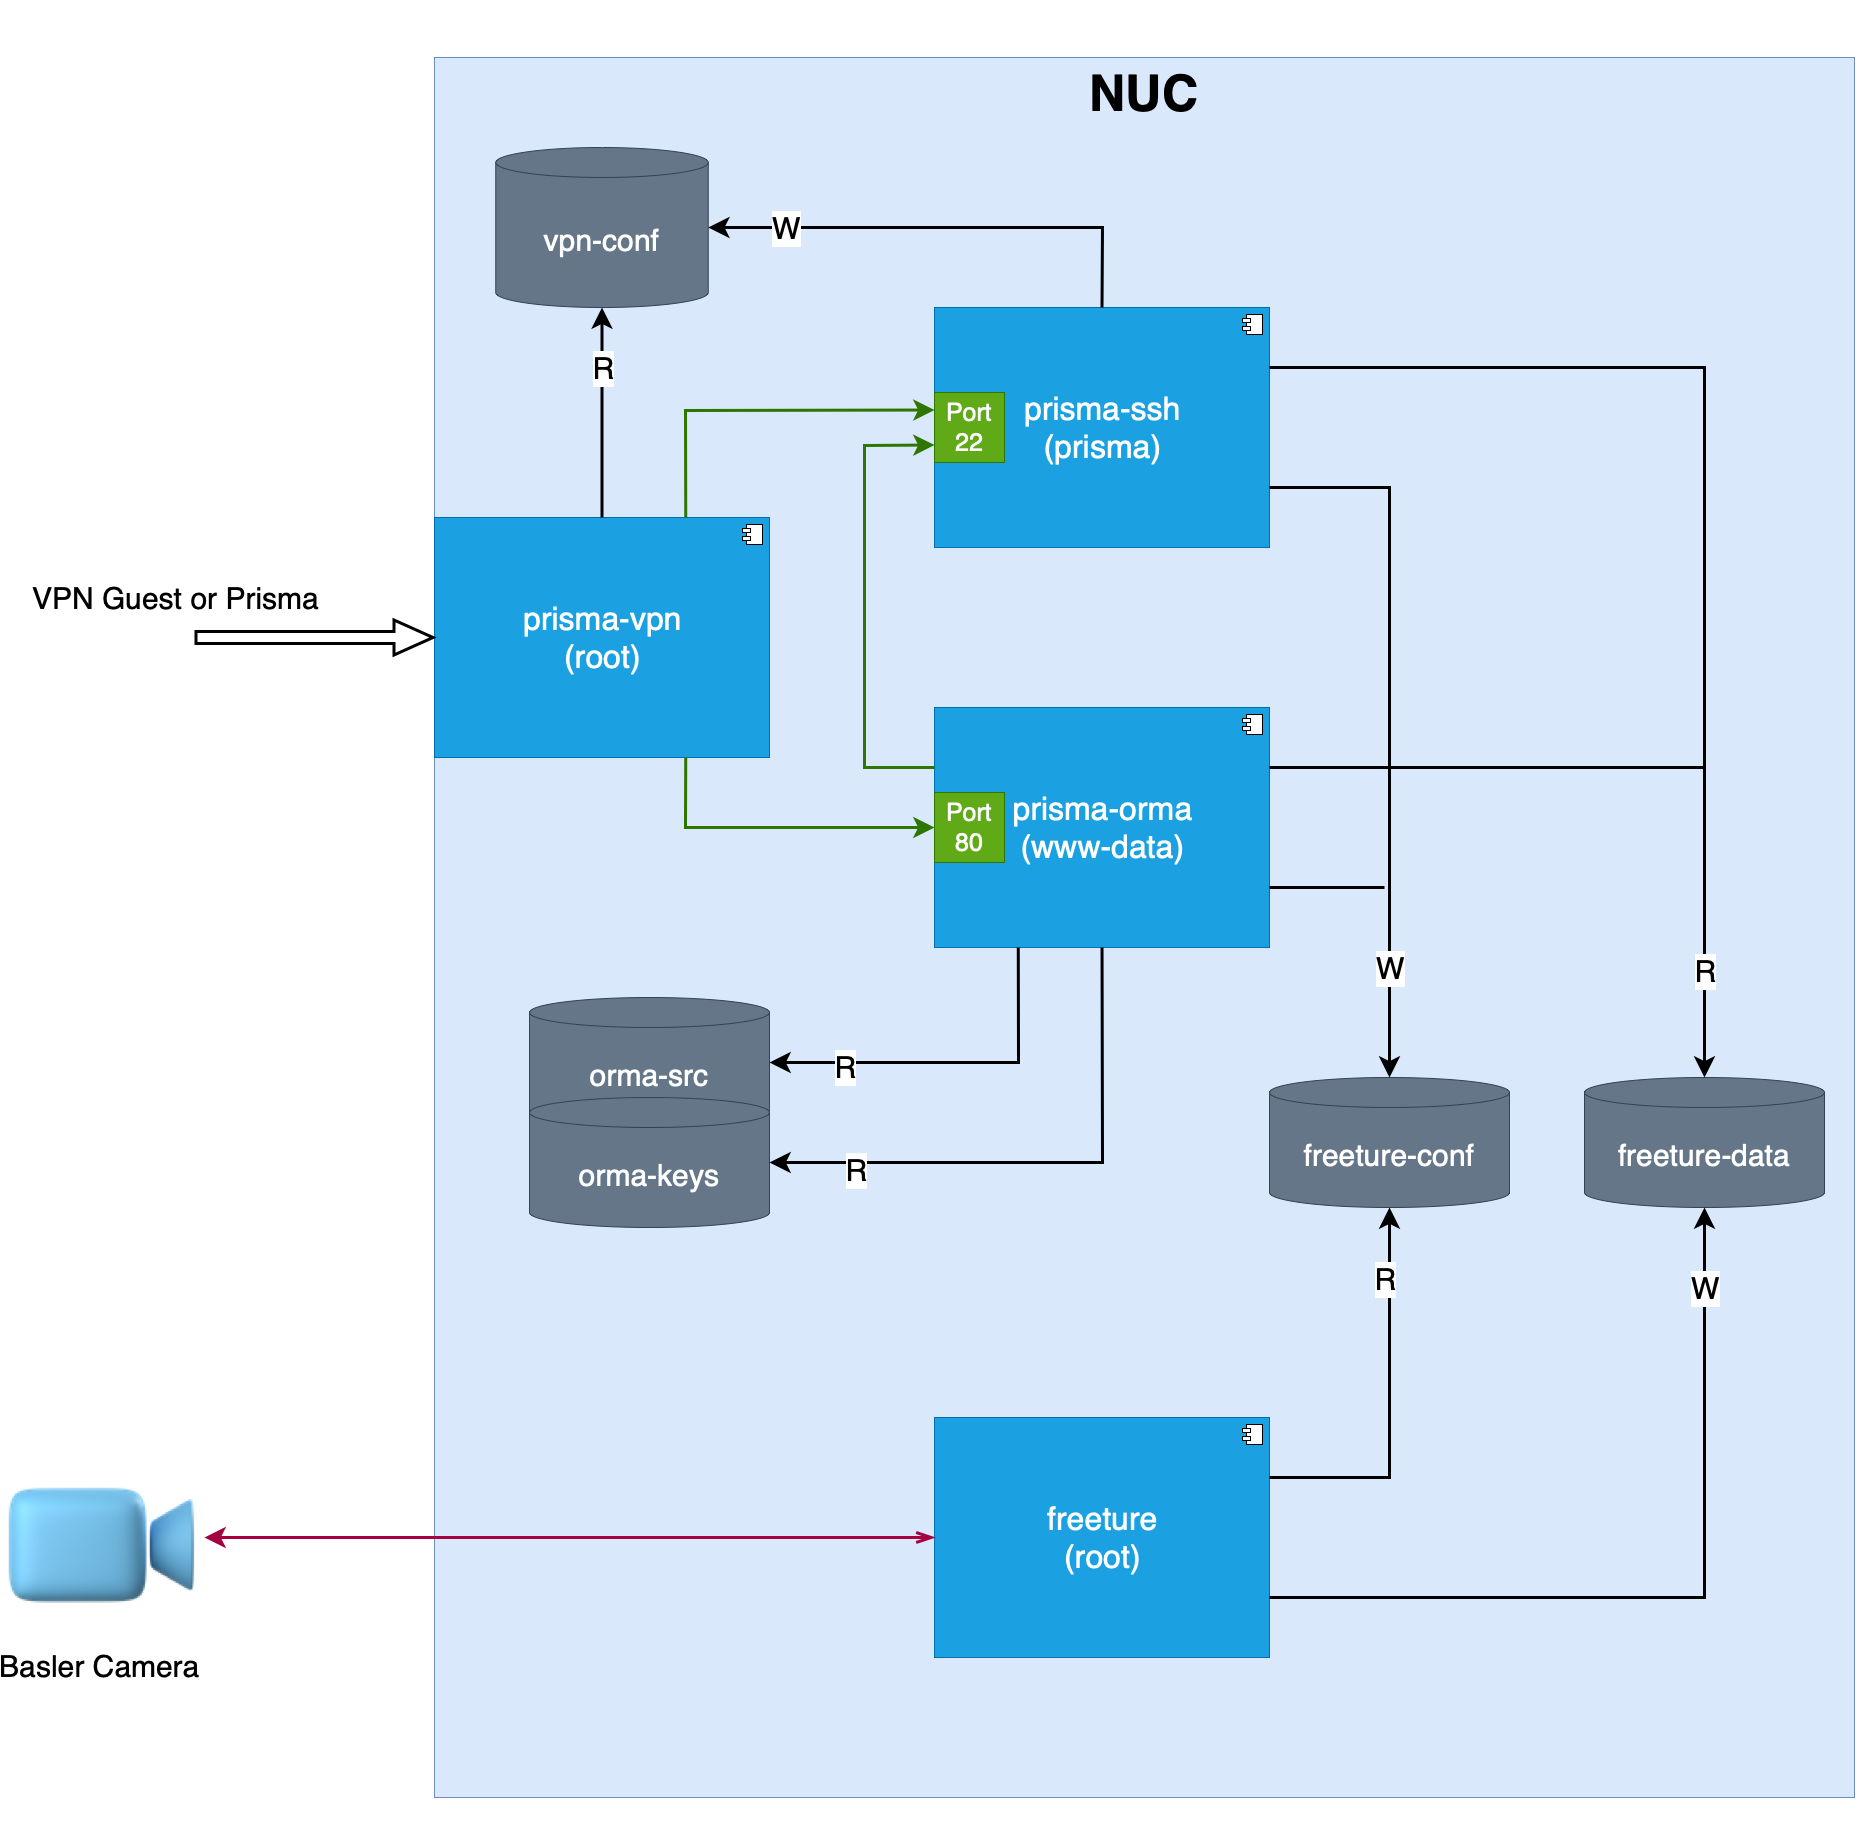
\includegraphics[width=\textwidth]{images/docker-arch.png} 
\caption{Visualizzazione grafica della struttura e delle interazioni dei container.}
\label{fig:containers-arch}
\end{center}
\end{figure}

\subsection{Struttura dati raccolti}

Nella sezione \ref{dati-raccolti} si sono presentati tre tipi di dati: \textbf{capture}, \textbf{stack} e \textbf{detection}. Nel volume \emph{freeture-data} vengono strutturati in una gerarchia ben definita, che verrà riproposta anche nell'interfaccia grafica della web application.

La struttura consta di una cartella per ciascun giorno, all'interno di ciascuna cartella sono presenti ulteriori tre cartelle, una per ogni tipo di dato. Le cartelle relative alle \emph{capture} e agli \emph{stack} sono popolate dai corrispondenti file FITS di quel giorno, mentre quella relativa delle \emph{detection} contiene a sua volta altre cartelle, ognuna coincidente con un evento nel giorno. Tra i file contenuti in quest'ultima cartella ai fini del lavoro svolto si denota la presenza dei fotogrammi, in formato FITS, che catturano la rilevazione, il file FITS principale e i file formato BMP DirMap e GeMap, versioni elaborate della rilevazione che evidenziano la porzione di cielo interessata dall'evento.

\subsection{Prometheus} \label{prometheus}

Le performance del nodo sono controllate tramite il software Prometheus \cite{Prometheus}, un insieme di strumenti per monitorare e notificare sistemi.

In particolar modo sulla macchina è configurato \emph{Prometheus Node Exporter}, che fornisce un'ampia varietà di metriche riguardo all'hardware e al kernel \cite{Prometheus-node-exporter}. Come già accennato, accedendo alla porta 9090 si può accedere all'interfaccia grafica fornita da Prometheus, per avere una panoramica generale delle performance della macchina. Le singole metriche sono invece fruibili sulla porta 9100.

La configurazione di Prometheus risiede sull'host in modo analogo alla VPN.

\begin{figure}[H] 
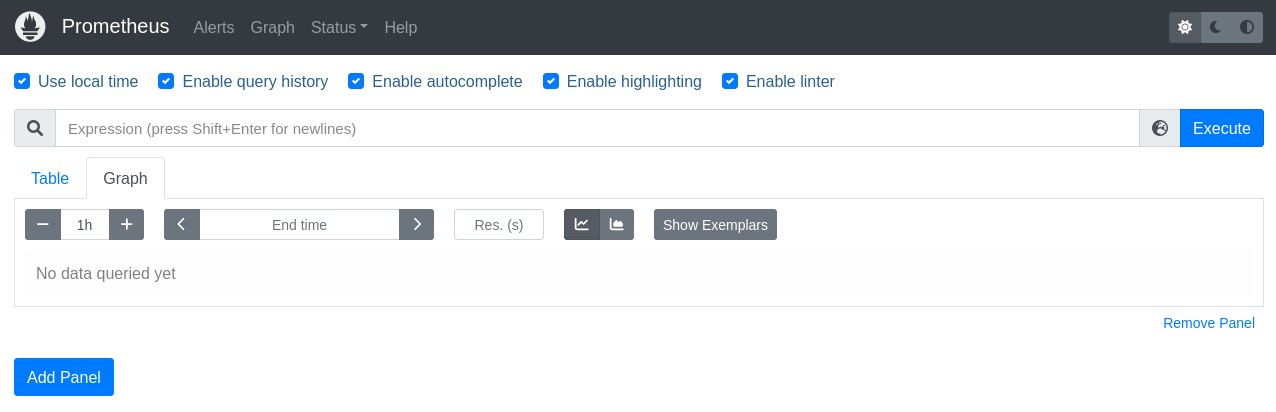
\includegraphics[width=\textwidth]{images/prometheus-9090.jpg} 
\caption{Interfaccia grafica di \emph{Prometheus Node Exporter}.}
\end{figure}